\section{Précision des systèmes asservis}

\subsection{Système non perturbé}
\marginnote{\textbf{Frédéric Mazet}, \textit{Cours d'automatique de deuxième année}, Lycée Dumont Durville, Toulon.}
\marginnote{\textbf{Florestan Mathurin}, \textit{Stabilité des SLCI}, Lycée Bellevue, Toulouse \url{http://florestan.mathurin.free.fr/}.}

\begin{defi}{}
La précision est l'écart entre la valeur de consigne et la valeur de la sortie. Pour caractériser la précision d'un système, on s'intéresse généralement à l'écart en régime permanent.

Attention à bien s'assurer que, lors d'une mesure expérimentale par exemple, les grandeurs de consigne et de sortie sont bien de la même unité (et qualifient bien la même grandeur physique).

\vspace{.2cm}

\noindent \begin{minipage}[c]{.6\linewidth}
Pour un système non perturbé dont le schéma-blocs est celui donné ci-contre, on caractérise l'écart en régime permanent par :
$$
\varepsilon_{\text{permanent}}=\lim\limits_{t\to +\infty} \varepsilon(t)
\quad
\Longleftrightarrow 
\quad
\varepsilon_{\text{permanent}}=\lim\limits_{p\to 0} p\varepsilon(p)
$$
\end{minipage}
\hspace{.5cm}
\begin{minipage}[c]{.25\linewidth}
%\includestandalone{Schema_1_entree_F_R}
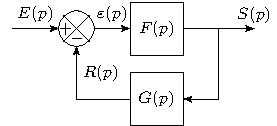
\includegraphics{Schema_1_entree_F_R}
\end{minipage}

\end{defi}

\begin{defi}{}
Un système est précis pour une entrée lorsque $\varepsilon_{\text{permanent}}=0$.
\end{defi}

\begin{defi}{} \~\\
Le nom de l'écart dépend de l'entrée avec lequel le système est sollicité : 
\begin{itemize}
\item écart statique, système sollicité par une entrée échelon : $e(t)=E_0$ et $E(p)=\dfrac{E_0}{p}$;
\item écart en vitesse ou en poursuite, système sollicité par une rampe : $e(t)=Vt$ et $E(p)=\dfrac{V}{p^2}$;
\item écart en accélération : système sollicité par une parabole, $e(t)=At^2$ et $E(p)=\dfrac{A}{p^3}$.
\end{itemize}
\end{defi}

\begin{center}
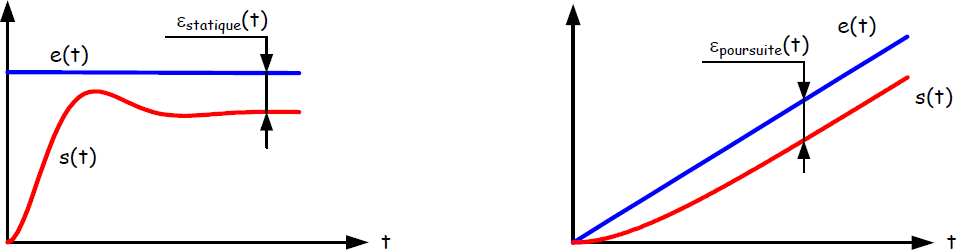
\includegraphics[width=.9\linewidth]{fig_erreur}
\end{center}

\subsection*{Petit développement ...}

Calculons l'écart statique pour le système précédent. On a : $\varepsilon(p)=E(p)-R(p)=E(p)-\varepsilon(p) F(p) G(p)$. En conséquences,
$\varepsilon(p)=E(p)-\varepsilon(p) F(p) G(p) 
\Longleftrightarrow \varepsilon(p)\left( 1+F(p) G(p) \right) =E(p) 
\Longleftrightarrow   \varepsilon(p) =\dfrac{E(p)}{1+F(p) G(p)}$.

\begin{resultat}
$$\varepsilon(p) =\dfrac{E(p)}{1+\text{FTBO}(p)}$$
\end{resultat}


\subsection*{Poursuivons ...}
On a $\text{FTBO}(p)=\dfrac{K_{BO}\left(1+a_1p+...+a_mp^m \right)}{p^{\alpha}\left(1+b_1p+...+b_np^n\right)}$ avec $m< n$.
\subsubsection*{FTBO de classe nulle}

\begin{itemize}
\item Pour une entrée échelon : 
$\varepsilon_{\text{perm}}=\lim\limits_{p\to 0} p\dfrac{E_0}{p}\dfrac{1}{1+\text{FTBO}(p)} 
= \dfrac{E_0}{1+K_{BO}}$.
\item Pour une entrée de type rampe : 
$\varepsilon_{\text{perm}}=\lim\limits_{p\to 0} p\dfrac{V}{p^2}\dfrac{1}{1+\text{FTBO}(p)} 
=+\infty$.
\item Pour une entrée de type parabole : 
$\varepsilon_{\text{perm}}=\lim\limits_{p\to 0} p\dfrac{A}{p^3}\dfrac{1}{1+\text{FTBO}(p)} 
=+\infty$.
\end{itemize}

\subsubsection*{FTBO de classe 1}

\begin{itemize}
\item Pour une entrée échelon : 
$\varepsilon_{\text{perm}}=\lim\limits_{p\to 0} p\dfrac{E_0}{p}\dfrac{1}{1+\dfrac{K_{BO}\left(1+a_1p+...+a_mp^m \right)}{p\left(1+b_1p+...+b_np^n\right)}} 
= 0$.
\item Pour une entrée de type rampe : 
$\varepsilon_{\text{perm}}=\lim\limits_{p\to 0} p\dfrac{V}{p^2}\dfrac{1}{1+\dfrac{K_{BO}\left(1+a_1p+...+a_mp^m \right)}{p\left(1+b_1p+...+b_np^n\right)}} 
=\dfrac{V}{K_{BO}}$.
\item Pour une entrée de type parabole : 
$\varepsilon_{\text{perm}}=\lim\limits_{p\to 0} p\dfrac{A}{p^3}\dfrac{1}{1+\dfrac{K_{BO}\left(1+a_1p+...+a_mp^m \right)}{p\left(1+b_1p+...+b_np^n\right)}} 
=+\infty$.
\end{itemize}

\subsubsection*{FTBO de classe 2}

\begin{itemize}
\item Pour une entrée échelon : 
$\varepsilon_{\text{perm}}=\lim\limits_{p\to 0} p\dfrac{E_0}{p}\dfrac{1}{1+\dfrac{K_{BO}\left(1+a_1p+...+a_mp^m \right)}{p^{2}\left(1+b_1p+...+b_np^n\right)}} 
= 0$.
\item Pour une entrée de type rampe : 
$\varepsilon_{\text{perm}}=\lim\limits_{p\to 0} p\dfrac{V}{p^2}\dfrac{1}{1+\dfrac{K_{BO}\left(1+a_1p+...+a_mp^m \right)}{p^{2}\left(1+b_1p+...+b_np^n\right)}} 
=0$.
\item Pour une entrée de type parabole : 
$\varepsilon_{\text{perm}}=\lim\limits_{p\to 0} p\dfrac{A}{p^3}\dfrac{1}{1+\dfrac{K_{BO}\left(1+a_1p+...+a_mp^m \right)}{p^{2}\left(1+b_1p+...+b_np^n\right)}} 
=\dfrac{A}{K_{BO}}$.
\end{itemize}


\begin{resultat} ~\\

\begin{center}
\begin{tabular}{|c|c|c|c|}
\hline 
Classe & Consigne échelon & Consigne en rampe & Consigne parabolique \\
& $e(t)=E_0$ & $e(t)=V t $ & $e(t)=At^2$ \\ 
& $E(p)=\dfrac{E_0}{p}$ & $E(p)=\dfrac{V}{p^2}$ & $E(p)=\dfrac{A}{p^3}$ \\ 
\hline \hline 
&&&\\
0 & $\varepsilon_S = \dfrac{E_0}{1+K_{BO}} $ & $\varepsilon_V = +\infty$ & $\varepsilon_A = +\infty$ \\
&&&\\
\hline 
&&&\\
1 & $\varepsilon_S = 0$ & $\varepsilon_V = \dfrac{V}{K_{BO}} $ & $\varepsilon_A = +\infty$ \\
&&&\\
\hline 
&&&\\
2 & $\varepsilon_S = 0 $ & $\varepsilon_V = 0$ & $\varepsilon_A = \dfrac{A}{K_{BO}}$ \\
&&&\\
\hline 
\end{tabular}
\end{center}

\begin{remarque}
L'écart statique est nul si la boucle ouverte comprend au moins une intégration. À défaut, l'augmentation du gain statique de la boucle ouverte provoque une amélioration de la précision.
\end{remarque}

\end{resultat}




%\begin{methode}[Détermination de l'erreur pour un système non perturbé]
%
%\end{methode}

%\begin{methode}[Détermination de l'erreur pour un système perturbé]
%
%\end{methode}
%
%\begin{resultat}
%Tableau...
%\end{resultat}

\subsection{Système perturbé}
Soit le schéma-blocs suivant : 
\begin{center}
%\includestandalone{Schema2Entrees_2F_R}
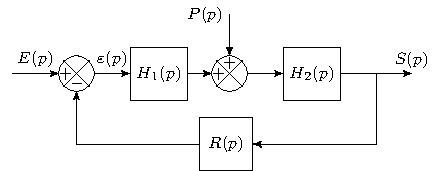
\includegraphics{Schema2Entrees_2F_R}
\end{center}

\vspace{.25cm}

\textbf{L'écart est caractérisé par le soustracteur principal, c'est-à-dire celui situé le plus à gauche du schéma-blocs.}

\vspace{.25cm}

Par lecture directe, on a : 
$\varepsilon(p)
=E(p)-R(p)S(p)
=E(p)-R(p)\left(H_2(p) \left(P(p)+\varepsilon(p)H_1(p) \right)\right)$
$\Longleftrightarrow 
\varepsilon(p) =E(p)- R(p)H_2(p)P(p)-R(p)H_1(p)H_2(p)\varepsilon(p) $
$\Longleftrightarrow \varepsilon(p)\left( 1+R(p)H_1(p)H_2(p)\right) =E(p)- R(p)H_2(p)P(p)$
$\Longleftrightarrow \varepsilon(p) =\dfrac{E(p)}{1+R(p)H_1(p)H_2(p)}- \dfrac{R(p)H_2(p)}{1+R(p)H_1(p)H_2(p)}P(p)$.

On a donc :
$\varepsilon(p) =\underbrace{\dfrac{1}{1+\text{FTBO}(p)} E(p)}_{\text{\'Ecart vis-à-vis de la consigne}} - \underbrace{\dfrac{R(p)H_2(p)}{1+\text{FTBO}(p)}P(p)}_{\text{\'Ecart vis-à-vis de la perturbation}}$.
%
%Notons $H_1(p)=\dfrac{K_1}{p^\alpha_1}\dfrac{N_1(p)}{D_1(p)}$ (avec $N_1(0)=1$ et $D_1(0)=1$) et $H_2(p)=\dfrac{K_2}{p^\alpha_2}\dfrac{N_2(p)}{D_2(p)}$ (avec $N_2(0)=1$ et $D_2(0)=1$).
%
%Par ailleurs 
%$H_{\text{bo}}(p)=H_1(p)H_2(p)R(p)
%=\dfrac{H_{\text{bo}}}{p^{\alpha}}\dfrac{N(p)}{D(p)}$.
%
%On peut calculer l'écart vis-à-vis de la perturbation : 
%$\varepsilon_{\text{perturbation}}
%= \lim\limits_{t\to\infty}\varepsilon(t)
%= \lim\limits_{p\to 0}p \varepsilon(p) 
%= \lim\limits_{p\to 0} \dfrac{K_2 p^{\alpha_1+1}}{p^{\alpha_1+\alpha_2}+K_1K_2}P(p) $.
%
%%$S(p)=H_2(p)\left(P(p)+H_1(p)\left(E(p)-R(p)S(p)\right) \right)$
%%$=P(p)H_2(p)+H_1(p)H_2(p)E(p)-H_1(p)H_2(p)R(p)S(p)$ 
%%$\Leftrightarrow S(p)\left( 1+H_1(p)H_2(p)R(p)\right)=P(p)H_2(p)+H_1(p)H_2(p)E(p)$
%%$\Leftrightarrow S(p)=P(p)\dfrac{H_2(p)}{1+H_1(p)H_2(p)R(p)}+\dfrac{H_1(p)H_2(p)}{1+H_1(p)H_2(p)R(p)}E(p)$.
%
%%On a donc $S(p)=P(p)\dfrac{H_2(p)}{1+\text{FTBO}(p)}+\dfrac{H_1(p)H_2(p)}{1+%\text{FTBO}(p)}E(p)$.
%\begin{center}
%\begin{tabular}{|c|c|c|}
%\hline
%Cas & Classe du système & Perturbation en échelon $P(p)=\dfrac{P_0}{p}$ \\ \hline
%1 & $\alpha_1\geq 1$ & $\varepsilon_{\text{perturbation}}=0$ \\ \hline
%2 & $\alpha_1=0$ et $\alpha_2=0$ & $\varepsilon_{\text{perturbation}}=\dfrac{K_2}{1+K_1K_2}P_0$ \\ \hline
%3 & $\alpha_1=0$ et $\alpha_2\geq 1$ & $\varepsilon_{\text{perturbation}}=\dfrac{P_0}{K_1}$ \\ \hline
%\end{tabular}
%\end{center}

\begin{resultat}
Il faut au moins un intégrateur en amont d'une perturbation constante pour
annuler l'écart vis-à-vis de cette perturbation. Un intégrateur placé en aval n'a aucune
influence.

Quand ce n'est pas le cas, un gain $K_1$ important en amont de la perturbation réduit toujours
l'écart vis-à-vis de cette perturbation.
\end{resultat}


\begin{center}
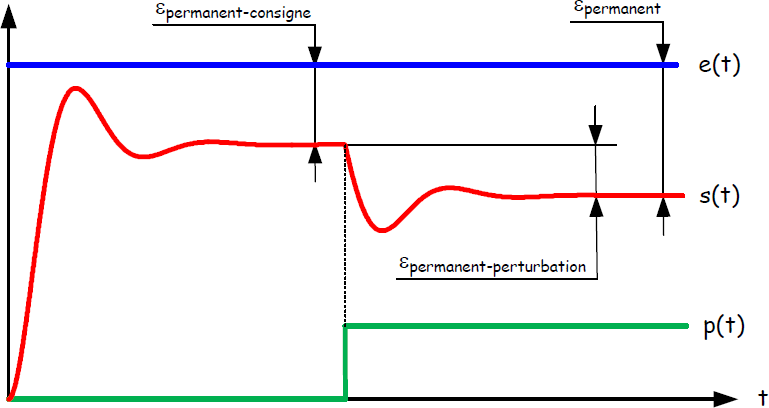
\includegraphics[width=.7\linewidth]{fig_erreur_02}
\end{center}


%\subsection{Précision et réponse fréquentielle}


%\begin{thebibliography}{2}
%   \bibitem[1]{ref1} Frédéric Mazet, {\it Cours d'automatique de deuxième année, Lycée Dumont Durville, Toulon.}
%      \bibitem[2]{ref2} Florestan Mathurin, {\it Précision des SLCI, Lycée Bellevue, Toulouse, \url{http://florestan.mathurin.free.fr/}.}
%
%\end{thebibliography}

%\end{document}



